\documentclass[12pt,a4paper]{article}
\usepackage[utf8]{inputenc}
\usepackage[portuguese]{babel}
\usepackage{amsmath}
\usepackage{amsfonts}
\usepackage{graphicx}
\usepackage{hyperref}
\usepackage{booktabs}
\usepackage{geometry}
\geometry{a4paper, margin=2.5cm}

\title{\textbf{Como estudar a arte usando redes?}\\ \large \textit{A Dinâmica de Influências na História da Arte}}
\author{Disciplina: SME5924 - Processos Dinâmicos em Redes Complexas \\ José Eduardo Saroba Bieco \\ \textbf{NUSP:} 15856890}
% \date{\today}

\begin{document}

\maketitle

\section{Introdução e Motivação}
\label{sec:introducao}

A história da arte é tradicionalmente estudada sob uma perspectiva linear e cronológica, organizada por períodos e movimentos estritamente delimitados. No entanto, a evolução estética e técnica é, fundamentalmente, um processo dinâmico impulsionado pela troca contínua de ideias e obras entre os indivíduos. Trabalhos pioneiros demonstraram que a história cultural pode ser mapeada quantitativamente como um sistema em evolução, evidenciando como a mobilidade e as conexões entre indivíduos formam redes de influência estruturadas ao longo dos séculos \cite{schich2014network}. Sob a ótica da ciência das redes, a adoção de um novo estilo ou vanguarda artística apresenta características análogas a fenômenos de contágio social e difusão de informação.

A aplicação de modelos de redes complexas em sistemas culturais demonstra que o desenvolvimento e o reconhecimento artístico são indissociáveis das interações estruturais da rede. Em áreas onde a avaliação de qualidade é subjetiva e carece de métricas absolutas, estudos empíricos indicam que a reputação e o acesso a nós e \textit{hubs} determinam fortemente a trajetória de sucesso e a visibilidade global de um artista e de suas obras, evidenciando uma dependência de caminho \cite{Fraiberger2018, jach2018quantifying}. Paralelamente, análises empíricas no ecossistema da música clássica revelam que a topologia dessas redes de influência é governada por um forte mecanismo de apego preferencial. Sob essa dinâmica, a capacidade de atrair novas conexões cresce de forma muito mais intensa para os nós mais consolidados, fazendo com que os grandes mestres concentrem uma quantidade altamente desproporcional de vínculos e moldem a evolução de todo o cenário cultural ao longo dos séculos \cite{park2015}.


Nesse contexto, o objetivo deste trabalho é modelar a história da arte global como uma rede complexa direcionada, onde os vértices representam os pintores e as arestas representam as relações diretas de influência (inspiração ou mestre-aprendiz). A partir da modelagem desta topologia, o estudo propõe três frentes de análise: (i) extrair métricas de centralidade e propriedades estruturais do grafo; (ii) identificar comunidades e correlacioná-las quantitativamente com os movimentos artísticos históricos; e (iii) aplicar os modelos epidêmicos SIR e SEIS para simular a propagação estocástica de estilos artísticos pela rede, avaliando matematicamente a dinâmica do contágio cultural.

\section{Materiais e Métodos}
\label{sec:materiais_metodos}

A modelagem de redes de influência exige bases de dados que explicitem conexões relacionais direcionadas. Fontes institucionais conhecidas, como o \textit{Museu de Arte Moderna} (MoMA), fornecem catálogos extensos, mas agrupam diversas mídias e carecem do mapeamento explícito de ``quem influenciou quem''. O uso de bases abertas como o Wikidata, por outro lado, demanda consultas em \textit{SPARQL} que dificultam a extração massiva e limpa das conexões desejadas.

Por essa razão, este projeto utiliza o dataset \textit{PainterPalette} \cite{painterpalette_ref}. A base estrutura variáveis biográficas, estilos e movimentos, fornecendo mapeamentos explícitos das influências recebidas e exercidas por milhares de artistas. Na etapa de pré-processamento, as colunas de estilo e movimento foram cunificadas para contornar a ausência de dados em registros isolados, resultando em um corpus coeso para a construção da topologia.

Bases de dados consolidadas a partir de múltiplas fontes abertas frequentemente apresentam ``ruídos''. Durante a construção inicial da rede, notou-se que o campo \texttt{influencias} continha rótulos genéricos (ex: \textit{male-portraits} e \textit{female-portraits}) que acabavam instanciados como vértices individuais. Visando preservar a integridade topológica e impedir que tais categorias atuassem artificialmente como \textit{hubs} de difusão, executou-se uma rotina de filtragem focada em remover relações que não envolvessem estritamente pintores reais. Contudo, em virtude da vasta diversidade de entradas textuais não estruturadas, reconhece-se a inviabilidade de uma supressão total destes artefatos, restando uma proporção residual de nós atípicos na topologia final.

\subsection{Modelagem da Rede}
\label{sec:modelagem}

O sistema foi modelado computacionalmente como um grafo direcionado $G = (V, E)$, operado através da biblioteca \texttt{networkx} em Python. O conjunto de vértices $V$ corresponde aos artistas, enquanto o conjunto de arestas $E$ representa o fluxo de conhecimento.

A direcionalidade constitui a premissa necessária para as simulações dinâmicas posteriores. Estabelece-se que o fluxo de informação parte do influenciador para o influenciado. Portanto, se o artista A exerceu influência sobre o artista B, a aresta é denotada como: $A \rightarrow B$.

O processo de instanciação e filtragem resultou em uma rede empírica com $|V| = 11.863$ nós e $|E| = 3.027$ arestas.

\subsection{Densidade Topológica}
\label{subsec:densidade}

Para aferir a conectividade global do sistema, avaliou-se a densidade da rede. A densidade de um grafo direcionado quantifica a razão entre o número de conexões existentes e o número máximo de conexões possíveis. Para um grafo com $V$ vértices e $E$ arestas, a densidade $D$ é dada por:

$$D = \frac{E}{V(V-1)}$$

Dado o tamanho da rede ($11.863$ nós), o número de arestas possíveis ultrapassa a marca de $140$ milhões (140.718.906). O cálculo da densidade resultou em $D \approx 2.2 \cdot 10^{-5}$. Este valor corrobora as expectativas de redes socioculturais e históricas: o grafo é extremamente esparso. Restrições geográficas e temporais impedem que um único pintor se conecte globalmente a todos os outros, limitando as interações a nichos locais e cronológicos. A dispersão da rede, caracterizada pela presença de um grande número de componentes desconectados e pela esparsidade extrema, pode ser observada visualmente na Figura \ref{fig:rede_geral}.

\begin{figure}[htpb]
    \centering
    \includegraphics[width=0.8\textwidth]{./figures/rede_completa.png}
    \caption{Visualização global da rede de influências artísticas original.}
    \label{fig:rede_geral}
\end{figure}

\section{Caracterização Topológica da Rede}
\label{sec:caracterizacao_rede}

Pesquisas recentes confirmam a viabilidade de aplicar teoria da informação e análises de aglomeração para quantificar a evolução de estilos complexos a partir de acervos digitais \cite{lee2020dissecting}, consolidando o uso de grandes bases de dados como uma ferramenta robusta para examinar a história da arte de forma orientada a dados (\textit{data-driven}). Seguindo essa mesma linha metodológica, calculamos as propriedades topológicas da nossa rede de pintores para compreender sua estrutura subjacente.

A caracterização de uma rede complexa inicia-se pela análise de suas propriedades macroscópicas. A Tabela \ref{tab:propriedades_globais} consolida as métricas globais extraídas tanto da rede empírica completa quanto do seu Maior Componente Fracamente Conectado (\textit{Weakly Connected Giant Component}) (Componente Gigante). A comparação evidencia o impacto da esparsidade extrema na rede como um todo e o ganho substancial de coesão, aglomeração e densidade quando isolamos o núcleo principal de influências históricas.

\begin{table}[htpb]
    \centering
    \caption{Propriedades topológicas globais da rede de influências artísticas comparadas ao seu Componente Gigante.}
    \label{tab:propriedades_globais}
    \begin{tabular}{@{}lcc@{}}
        \toprule
        \textbf{Métrica}                             & \textbf{Rede Completa}  & \textbf{Componente Gigante} \\ \midrule
        Número de Nós ($N$)                          & 11.863                  & 1.428                       \\
        Número de Arestas ($E$)                      & 3.027                   & 2.322                       \\
        Grau Médio Direcionado ($\langle k \rangle$) & $2.55 \times 10^{-1}$   & $1.626$                     \\
        Densidade ($D$)                              & $2.20 \times 10^{-5}$   & $1.14 \times 10^{-3}$       \\
        Transitividade                               & $9.60 \times 10^{-3}$   & $9.60 \times 10^{-3}$       \\
        Aglomeração Média ($C$)                      & $2.10 \times 10^{-3}$   & $1.67 \times 10^{-2}$       \\
        Assortatividade                              & $-1.752 \times 10^{-1}$ & $-1.721 \times 10^{-1}$     \\ \bottomrule
    \end{tabular}
\end{table}

A distribuição de conectividade dita a resiliência e a dinâmica de propagação de um grafo. Redes de influência cultural frequentemente assumem uma topologia Livre de Escala (\textit{Scale-Free}), onde a distribuição da probabilidade de grau decai segundo uma lei de potência ($P(k) \sim k^{-\gamma}$) \cite{barabasi_network_science, park2015}.

Para validar esta hipótese, utilizou-se a Estimativa de Máxima Verossimilhança (MLE) via biblioteca \texttt{powerlaw}. A estimativa inicial para o grau de saída apontou um expoente $\gamma \approx 2.46$. No entanto, o teste de robustez via \textit{Loglikelihood Ratio} ($R = -5.4639$, $p$-valor $\approx 4.65 \times 10^{-8}$) demonstrou que uma distribuição Lognormal ajusta-se de forma estatisticamente superior aos dados empíricos em comparação à Lei de Potência pura. Ainda que a distribuição seja Lognormal, a presença de uma cauda pesada, evidenciada visualmente na Figura \ref{fig:dist_grau}, confirma a existência de \textit{hubs} super-espalhadores de tendências artísticas.

\begin{figure}[htpb]
    \centering
    \includegraphics[width=0.8\textwidth]{./figures/dist_grau.png}
    \caption{Distribuição empírica do grau de saída (\textit{Out-Degree}) em escala \textit{log-log}. O decaimento em cauda pesada ilustra a topologia fortemente assimétrica da rede: a imensa maioria dos artistas exerce pouca influência direta, enquanto uma seleta minoria (\textit{hubs}) irradia tendências para uma grande parcela do sistema.}
    \label{fig:dist_grau}
\end{figure}

\subsection{Métricas de Centralidade e Influência}
\label{subsec:metricas}

Para quantificar a importância individual de cada pintor, quatro métricas topológicas fundamentais foram computadas:
\begin{itemize}
    \item \textbf{Grau de Entrada (\textit{In-Degree}):} Mede a suscetibilidade do nó. Altos valores indicam pintores que absorveram técnicas de múltiplas fontes.
    \item \textbf{Grau de Saída (\textit{Out-Degree}):} Mede o alcance direto. \textit{Hubs} neste critério são grandes difusores de tendências.
    \item \textbf{\textit{PageRank}:} Diferentemente do grau, o \textit{PageRank} não avalia apenas a quantidade, mas a qualidade das conexões. Um artista pontua alto se influenciou outros nomes canônicos\footnotemark \footnotetext{Refere-se aos artistas tradicionais e amplamente consagrados pela história da arte.} da rede.
    \item \textbf{Intermediação (\textit{Betweenness}):} Identifica pontes. Artistas com alta intermediação são gargalos por onde um estilo transita entre gerações ou comunidades distintas.
\end{itemize}

A Tabela \ref{tab:centralidades} ilustra o comportamento destas métricas para artistas de destaque na rede já filtrada. \textit{Isaac Levitan} demonstra altíssima centralidade em todos os quesitos, atuando tanto como um grande absorvedor (\textit{In-Degree} de 156) quanto como um pilar canônico (\textit{PageRank} de $9.32 \times 10^{-3}$). A coerência destes resultados atesta a necessidade fundamental da filtragem inicial de dados (\autoref{sec:materiais_metodos}): testes prévios com a rede não-filtrada revelaram que artefatos do \textit{dataset}, como \textit{male-portraits}, alcançavam graus de saída superiores aos de muitos pintores reais. Sem o devido tratamento, essas categorias genéricas agiriam topologicamente como falsos \textit{hubs} de difusão, distorcendo as métricas de influência e corrompendo a representatividade do sistema.

\begin{table}[htpb]
    \centering
    \caption{Métricas de centralidade computadas.}
    \label{tab:centralidades}
    \begin{tabular}{@{}lcccc@{}}
        \toprule
        \textbf{Nó / Vértice} & \textbf{In-Degree} & \textbf{Out-Degree} & \textbf{PageRank}     & \textbf{Betweenness}  \\ \midrule
        Isaac Levitan         & 156                & 118                 & $9.32 \times 10^{-3}$ & $1.26 \times 10^{-3}$ \\
        Alexander Ivanov      & 1                  & 55                  & $1.13 \times 10^{-4}$ & $8.41 \times 10^{-4}$ \\
        Umberto Boccioni      & 4                  & 48                  & $2.72 \times 10^{-4}$ & $3.79 \times 10^{-4}$ \\
        Paul Cezanne          & 6                  & 20                  & $2.38 \times 10^{-4}$ & $3.4 \times 10^{-5}$  \\
        Caravaggio            & 2                  & 18                  & $9.7 \times 10^{-5}$  & $6.0 \times 10^{-6}$  \\ \bottomrule
    \end{tabular}
\end{table}

\subsection{Transitividade e Assortatividade}
\label{subsec:transitividade}

A transitividade global da rede é baixa ($9.6 \times 10^{-3}$), e o coeficiente de aglomeração médio resulta em $2.1 \times 10^{-3}$. No contexto histórico, isso indica que ``triângulos'' fechados de influência são raros. Essa característica é complementada pelo Coeficiente de Assortatividade negativo ($-0.1752$). Uma rede desassortativa revela um comportamento estritamente hierárquico na transmissão do conhecimento: grandes mestres (\textit{hubs} de altíssimo grau) tendem a influenciar majoritariamente uma massa de aprendizes de baixo grau.

\section{Componente Gigante e Comunidades}
\label{sec:componente_gigante}

Devido à vasta extensão espaço-temporal da história da arte, a rede original fragmenta-se em diversas ilhas de conexões isoladas. A prova matemática dessa dispersão reside no fato de que o Maior Componente Fracamente Conectado concentra $1.428$ nós (apenas $12.0$\% da rede original) e $2.322$ arestas. A topologia deste núcleo exibe propriedades clássicas de Pequeno Mundo (\textit{Small-World}) (\autoref{sec:modelos_nulos}). O diâmetro máximo encontrado foi de $13$ saltos, com um caminho mais curto médio de $5.43$. Isso sugere que, apesar das barreiras de época, qualquer inovação estética desenvolvida na história da arte europeia poderia alcançar qualquer outro pintor na rede principal em menos de $5$ ``graus de separação''.

\subsection{Detecção de Comunidades e a Descentralização dos Movimentos}

O algoritmo de \textit{Louvain} foi aplicado para otimizar a modularidade do grafo, atingindo um valor expressivo de $Q = 0.7278$ (dividido em 17 comunidades principais no componente gigante). Este índice indica uma estrutura comunitária forte, onde as influências ocorrem primariamente de forma intragrupo, caracterizando a coesão local de ateliês ou escolas artísticas (``panelinhas''). A Figura \ref{fig:comunidades_louvain} ilustra espacialmente a segregação topológica e a densidade destas partições dentro do Componente Gigante.

Um resultado notável desta etapa é a identificação matemática da fragmentação de movimentos artísticos reais. Comunidades estruturalmente independentes apresentaram rótulos predominantes idênticos, como o \textit{Art Nouveau} e o \textit{Cubism}.

Como o método de \textit{Louvain} opera estritamente sobre a densidade topológica das arestas (sendo cego aos atributos semânticos dos vértices), esta fragmentação não constitui um erro de clusterização, mas uma descoberta analítica sobre a descentralização do contágio artístico. O Barroco, por exemplo, bifurca-se topologicamente entre as tradições Católica e Protestante. Esses grupos se desenvolveram simultaneamente sob o mesmo rótulo estilístico, porém isolados por barreiras geográficas e religiosas, resultando em bacias de influência topologicamente separadas.

\begin{figure}[htpb]
    \centering
    \includegraphics[width=0.9\textwidth]{./figures/g_gigante-comunidades.png}
    \caption{Grafo direcionado do Componente Gigante colorido pelas partições detectadas pelo algoritmo de Louvain.}
    \label{fig:comunidades_louvain}
\end{figure}

\section{Processos Dinâmicos de Influência}

A difusão de inovações estéticas e o surgimento de vanguardas podem ser tratados matematicamente como processos epidêmicos. A literatura estabelece que a adoção de um movimento ou técnica segue dinâmicas de infecção temporal e espacial, onde indivíduos tornam-se ``suscetíveis'', são expostos à ideia por meio do contato na rede, e podem eventualmente abandoná-la \cite{bettencourt2006power}. Baseando-se nessa premissa, modelamos a transmissão de um estilo artístico utilizando os processos SIR e SEIS.

Tradicionalmente, os modelos epidemiológicos clássicos assumem populações perfeitamente misturadas, com dinâmicas de campo médio comumente regidas por sistemas de Equações Diferenciais Ordinárias (EDOs). No contexto deste trabalho, essa premissa é descartada: a nossa implementação computacional transpõe essa lógica para o nível microscópico da rede. Assim, a dinâmica é modelada como um processo estocástico de tempo discreto, cuja probabilidade de transição temporal é estritamente governada pela matriz de adjacência $A_{ij}$ do grafo e pela vizinhança local de cada vértice \cite{ndlib_ref}.

\subsection{O Modelo SIR no Recorte Temporal (1850-1920)}

O modelo SIR (Suscetível-Infectado-Removido) clássico, na sua formulação contínua e homogénea, é regido pelo seguinte sistema de equações diferenciais ordinárias:
\begin{align}
    \frac{dS}{dt} & = -\beta \frac{S I}{N}           \\
    \frac{dI}{dt} & = \beta \frac{S I}{N} - \gamma I \\
    \frac{dR}{dt} & = \gamma I
\end{align}

Na abordagem estruturada em rede, a probabilidade de um pintor suscetível $i$ adotar uma nova tendência no instante $t$ depende exclusivamente da sua vizinhança direta, sendo calculada por $P(S_i \to I_i) = 1 - (1 - \beta)^{m_i}$, onde $m_i$ representa o número de influenciadores diretos de $i$ que estão infetados, e $\beta = 0.15$ dita a taxa de contágio empírica. A transição espontânea para o estado removido (abandono do estilo ou falecimento) ocorre com probabilidade $\gamma = 0.05$.

Para observar esta difusão em tempo real entre artistas que efetivamente coexistiram, isolou-se um recorte temporal de forte ``efervescência artística'' (1850 a 1920), contendo 236 nós e 433 arestas. A Figura \ref{fig:sir_simulacao} ilustra a evolução temporal deste processo. Como esperado no modelo SIR, observa-se o esgotamento natural da epidemia cultural à medida que a população infetada transita definitivamente para o estado de imunidade ou inatividade ($R$).

\begin{figure}[htpb]
    \centering
    \includegraphics[width=0.9\textwidth]{./figures/sir_simulacao.png}
    \caption{Simulação do Modelo SIR: Propagação do estilo artístico ao longo de 200 iterações no recorte temporal de 1850-1920.}
    \label{fig:sir_simulacao}
\end{figure}

\subsection{O Modelo SEIS}

Uma limitação do modelo SIR clássico, quando aplicado a fenômenos socioculturais, é a premissa da imunidade permanente (o estado $R$). Na história da arte, artistas frequentemente possuem ``fases'' e podem revisitar estilos do passado ou abandonar uma vanguarda para voltar a ser influenciados por outras tendências. Para capturar essa dinâmica cíclica, somada ao tempo inerente de assimilação de uma técnica, aplicamos o modelo SEIS (Suscetível-Exposto-Infectado-Suscetível).

Sob a aproximação clássica de campo médio para populações homogêneas, a dinâmica contínua do modelo é descrita pelo seguinte sistema de EDOs:
\begin{align}
    \frac{dS}{dt} & = -\beta \frac{S I}{N} + \lambda I \\
    \frac{dE}{dt} & = \beta \frac{S I}{N} - \alpha E   \\
    \frac{dI}{dt} & = \alpha E - \lambda I
\end{align}

No entanto, em uma abordagem estruturada por redes complexas, o processo se torna estocástico e de tempo discreto, sendo estritamente condicionado à vizinhança topológica de cada pintor. As transições de estado para cada nó $i$ no instante $t$ obedecem às seguintes probabilidades e regras analíticas:

\begin{itemize}
    \item \textbf{$S \to E$ (Suscetível para Exposto):} Ocorre por meio do contágio direcional. A probabilidade de um nó suscetível $i$ ser exposto e entrar na fase de latência é formulada por $P(S_i \to E_i) = 1 - (1 - \beta)^{m_i}$, onde $m_i$ representa o número de vizinhos diretos (influenciadores) de $i$ que estão no estado Infectado ($I$) no tempo $t$ e $\beta = 0.15$.
    \item \textbf{$E \to I$ (Exposto para Infectado):} O término do período latente — que representa empiricamente o intervalo de estudo e assimilação da nova técnica — ocorre de forma espontânea com uma probabilidade constante por unidade de tempo definida por $P(E_i \to I_i) = \alpha = 0.02$.
    \item \textbf{$I \to S$ (Infectado para Suscetível):} Representa a ``mudança de fase'' do artista. O abandono temporal do estilo e o consequente retorno ao estado de suscetibilidade (aberto a novas inspirações) ocorre com probabilidade constante $P(I_i \to S_i) = \lambda = 0.05$.
\end{itemize}

A simulação no mesmo recorte temporal de 1850-1920 (Figura \ref{fig:seis_simulacao}) revela uma sustentação endémica e oscilações no número de artistas ativos por estilo. Este comportamento valida a hipótese de que a produção artística possui uma fluidez não-definitiva superiormente representada pela estrutura cíclica do SEIS.

\begin{figure}[htpb]
    \centering
    \includegraphics[width=0.9\textwidth]{./figures/seis_simulacao.png}
    \caption{Simulação do Modelo SEIS: Evolução da dinâmica cíclica e do período de latência na arte ao longo de 200 iterações no recorte temporal (1850-1920).}
    \label{fig:seis_simulacao}
\end{figure}

\subsection{Simulação Global}

Por fim, expandiu-se a análise de propagação para a totalidade da rede através do Componente Gigante. Conceitualmente, o fluxo de influências deveria comportar-se naturalmente como um Grafo Direcionado Acíclico (DAG), fluindo estritamente do passado para o futuro. No entanto, bases de dados empíricas carregam ruídos, citações póstumas e ciclos de influência mútua entre contemporâneos. Estas inconsistências criam anomalias estruturais onde o futuro aparenta influenciar o passado ou onde a propagação fica retida em laços cíclicos fechados.

Para garantir a ``seta do tempo'' e viabilizar a simulação geracional ao longo de séculos, a topologia global foi submetida a um algoritmo de filtragem cronológica. Esta rotina computacional avaliou o ano de nascimento e de falecimento de cada par de pintores conectados por uma aresta ($u \to v$). Como critério de corte, a conexão foi removida caso os artistas houvessem coexistido em qualquer momento (sobreposição do tempo de vida) ou caso houvesse ausência de dados biográficos para qualquer um dos nós, evitando ciclos acidentais.

Esta restrição assegura que a influência flua estritamente ``para a frente'' na história, representando a transmissão de conhecimento entre gerações distintas. A aplicação deste filtro resultou na remoção de $3.029$ arestas anómalas. Em seguida, extraiu-se o novo maior componente fracamente conectado, convertendo o grafo num DAG puro e garantindo a sua conectividade para a simulação em larga escala.

Com a estrutura cronológica corrigida, executaram-se os modelos epidemiológicos para observar o comportamento do contágio ao longo de 200 iterações. A ausência de ciclos no DAG provou ter um impacto severo na sustentação das vanguardas. Ao aplicar o modelo SIR, a propagação extinguiu-se rapidamente: na iteração 50, contabilizaram-se 12 infetados ($I$) e 51 recuperados ($R$); contudo, já na iteração 100, a epidemia encontrava-se totalmente erradicada ($I = 0$, mantendo-se estática até ao final com 63 pintores que adotaram e abandonaram a técnica).

Em contraste, a aplicação do modelo SEIS na mesma topologia (Figura \ref{fig:seis_global}) demonstrou uma sobrevida maior da influência devido ao período de latência (estado $E$). Na iteração 50, o sistema registou 31 nós expostos e 10 infetados. Ao longo da simulação, a onda de contágio desceu pelas linhagens de forma decrescente: na iteração 100 ($E = 17$, $I = 6$) e, finalmente, na iteração 200, a propagação perdeu quase toda a sua força, resultando em apenas 5 expostos e 7 infetados num universo de 1.416 suscetíveis.

Estes resultados quantitativos validam uma premissa histórica: em um sistema estritamente linear (sem laços de retroalimentação ou revisitação ao passado), um estilo flui como uma onda unidirecional e inevitavelmente decai rumo ao esquecimento. A perpetuidade das vanguardas depende, portanto, da efervescência paralela e das trocas mútuas que os modelos cíclicos conseguem capturar nas redes contemporâneas.

\begin{figure}[htpb]
    \centering
    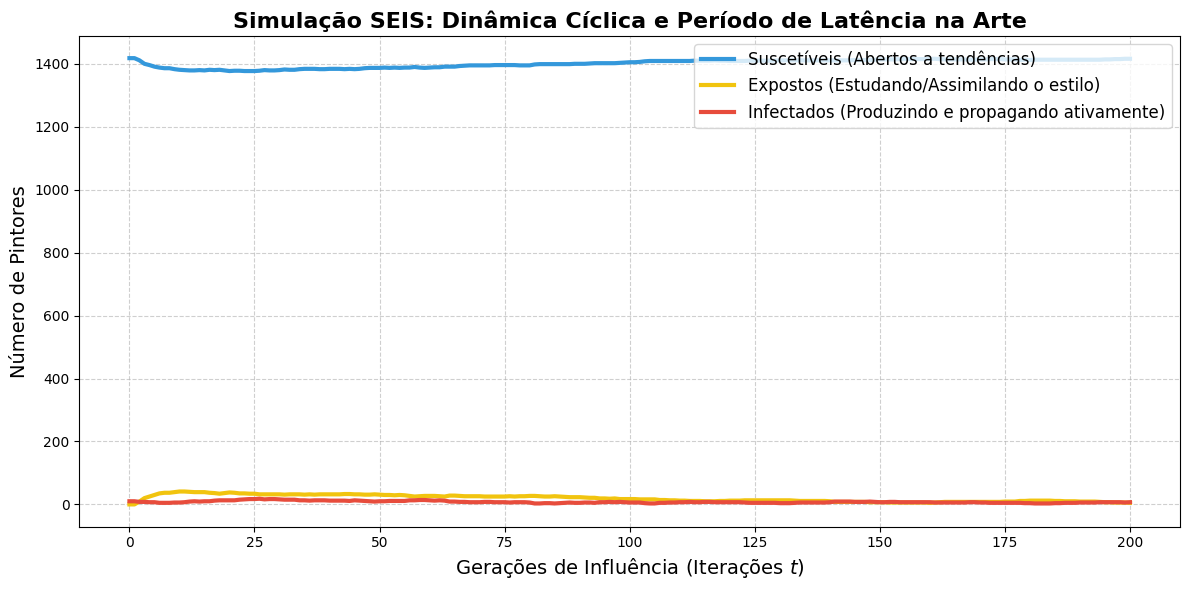
\includegraphics[width=0.9\textwidth]{./figures/dag_seis.png}
    \caption{Evolução dos estados Suscetível ($S$), Exposto ($E$) e Infetado ($I$) no modelo SEIS aplicado ao DAG.}
    \label{fig:seis_global}
\end{figure}

\section{Validação Estatística com Modelos Nulos}
\label{sec:modelos_nulos}
Para atestar que as propriedades estruturais observadas (alta aglomeração e distâncias curtas) possuem significado sociológico e não são fruto do acaso, a rede real foi comparada a três modelos nulos (Tabela \ref{tab:modelos_nulos}) gerados sobre o componente gigante não-direcionado \cite{barabasi_network_science, newman_networks}.

\begin{table}[htpb]
    \centering
    \caption{Comparação de métricas globais entre a rede real de arte e os modelos nulos.}
    \label{tab:modelos_nulos}
    \begin{tabular}{@{}lcccc@{}}
        \toprule
        \textbf{Métrica}    & \textbf{Rede Real}    & \textbf{Erdős-Rényi} & \textbf{Configuração} & \textbf{Barabási-Albert} \\ \midrule
        Caminho Médio ($L$) & 5.4309                & 6.2374               & 4.1823                & 4.2371                   \\
        Aglomeração ($C$)   & $3.27 \times 10^{-2}$ & $2.1 \times 10^{-3}$ & $1.83 \times 10^{-2}$ & $2.05 \times 10^{-2}$    \\ \bottomrule
    \end{tabular}
\end{table}

A análise comparativa, corroborada pela projeção espacial dos grafos ilustrada na Figura \ref{fig:modelos_nulos}, permite classificar a rede de influências da arte sob dois comportamentos topológicos:

\begin{enumerate}
    \item \textbf{Rede de Pequeno Mundo (\textit{Small-World}):} O coeficiente de aglomeração da rede real ($C = 3.27 \times 10^{-2}$) é quase quinze vezes superior ao esperado por uma distribuição puramente aleatória via Erdős-Rényi ($C_{ER} = 2.1 \times 10^{-3}$). Simultaneamente, o caminho mais curto ($L = 5.4309$) mantém-se pequeno, inclusive inferior ao limite aleatório ($L_{ER} = 6.2374$). Isso comprova estatisticamente a forte coesão local combinada a uma rápida capacidade de transmissão global.

    \item \textbf{Dinâmica de Apego Preferencial:} A topologia real converge expressivamente para os modelos de Configuração e Barabási-Albert (BA). A aproximação com as métricas do modelo BA ($L_{BA} = 4.2371$, $C_{BA} = 2.05 \times 10^{-2}$) valida que o mecanismo subjacente à história da arte é o apego preferencial (``o rico fica mais rico''). A influência não se distribui ao acaso; ela concentra-se em grandes mestres cujo peso histórico atrai desproporcionalmente as conexões (atenção e estudo) de novas gerações de aprendizes. Essa convergência é visualmente notória na Figura \ref{fig:modelos_nulos}, onde a rede real e o modelo BA exibem a mesma assinatura topológica: núcleos densos concentrados em poucos super-espalhadores, em forte contraste com a malha dispersa e homogênea do modelo aleatório.
\end{enumerate}

\begin{figure}[htpb]
    \centering
    \includegraphics[width=\textwidth]{./figures/modelos_nulos.png}
    \caption{Comparação topológica visual entre um subgrafo representativo da rede real de arte e as topologias sintéticas equivalentes geradas pelos modelos nulos. O dimensionamento dos vértices é proporcional ao seu respectivo grau. A representação evidencia a falha do modelo de Erdős-Rényi em capturar a heterogeneidade do sistema, contrastando com o notável alinhamento estrutural entre a rede real e o modelo de Barabási-Albert na formação de \textit{hubs} centrais.}
    \label{fig:modelos_nulos}
\end{figure}

\section{Conclusão}

A modelagem da história da arte como uma rede complexa demonstrou que a evolução estética não se restringe a uma progressão estritamente cronológica, comportando-se matematicamente como um processo de difusão de conhecimento governado por regras topológicas definidas. A análise estrutural confirmou que o fluxo de influências opera sob uma dinâmica de apego preferencial. A validação contra o modelo de BA justifica a topologia hierárquica e desassortativa do sistema: uma minoria de grandes mestres atrai de forma assimétrica a atenção das novas gerações, atuando como super-espalhadores de conhecimento.

Além disso, a abstração matemática foi capaz de redescobrir fenômenos histórico-geográficos de forma cega. A detecção de comunidades otimizou a rede e mapeou a descentralização de movimentos como o Barroco, isolando vertentes desenvolvidas paralelamente, porém separadas por barreiras religiosas e espaciais. A necessidade de filtragem rigorosa para a construção do DAG evidenciou que a modelagem topológica não substitui a historiografia da arte, exigindo uma leitura crítica que alinhe as abstrações matemáticas aos dados empíricos e à restrição imposta pela física do tempo.

No âmbito dos processos dinâmicos, a simulação revelou que epidemias culturais são descritas com maior precisão pelo modelo SEIS do que pelo clássico SIR. A adoção de um período de latência e a remoção da premissa de imunidade permanente capturam de forma mais realista o tempo necessário para a assimilação de uma técnica e a fluidez intrínseca às fases da carreira de um pintor. Em suma, os resultados obtidos validam quantitativamente a hipótese de que a sucessão de vanguardas na arte obedece a propriedades estruturais mensuráveis, oferecendo uma integração entre a ciência de redes e a sociologia cultural.

Apesar destes resultados, a abstração impõe limitações inerentes. Primeiramente, as arestas de influência foram tratadas de forma binária e não-ponderada (\textit{unweighted}). Na realidade, a força da transmissão varia substancialmente entre a tutela formativa de um mestre sobre o seu aprendiz e a mera observação pontual de um trabalho contemporâneo. Adicionalmente, ressalta-se o viés geográfico e historiográfico das bases de dados abertas, que favorecem desproporcionalmente a arte eurocêntrica. Este desbalanceamento pode atuar como um fator de influência na forte aglomeração do Componente Gigante e na fragmentação excessiva das bacias artísticas periféricas.

Como desdobramento para trabalhos futuros, destaca-se a oportunidade de inferir os parâmetros do modelo SEIS diretamente de estilos históricos reais, utilizando técnicas de aprendizado de máquina ou otimização inversa para calibrar o modelo de forma empírica. Por fim, a exploração de diferentes perfis epidemiológicos permitiria simular o impacto de vanguardas variadas. Enquanto os parâmetros adotados neste estudo testaram uma conjuntura conservadora e efêmera ($\alpha = 0.02$ e $\lambda = 0.05$), a aplicação do modelo a um estilo ``altamente desejável'' — caracterizado por alta e rápida assimilação e baixíssima taxa de abandono — ofereceria uma fundamentação matemática exata para diferenciar movimentos passageiros de vanguardas que moldaram o rumo da história.

\section*{Disponibilidade de Código}
O código completo da implementação, pré-processamento e simulações está disponível em: \url{https://github.com/JoseBieco/painterPallet-network-dynamics}.

\renewcommand{\refname}{Referências}
\bibliographystyle{unsrt}
\bibliography{referencias}

\end{document}